\begin{center}
    \textbf{Geração 40}
\end{center}

\begin{figure}[h]
    \centering
    \label{fig:geracaoXX}
    
    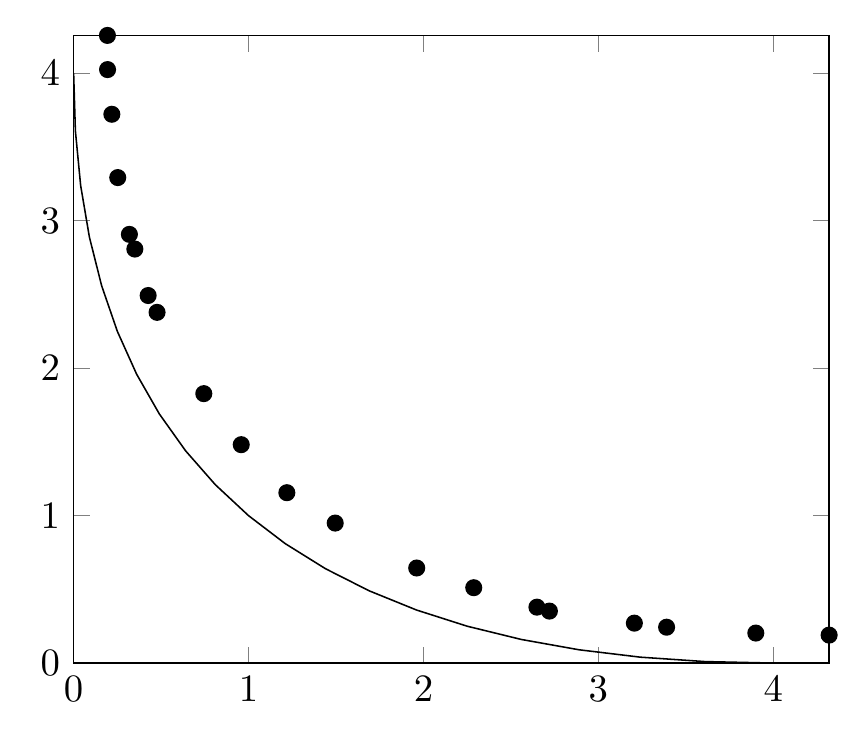
\begin{tikzpicture}[scale=1.4]
        \begin{axis}[enlargelimits=false]
            \addplot [] coordinates {
                (0.000000,4.000000) (0.010000,3.610000) (0.040000,3.240000) (0.090000,2.890000) (0.160000,2.560000) (0.250000,2.250000) (0.360000,1.960000) (0.490000,1.690000) (0.640000,1.440000) (0.810000,1.210000) (1.000000,1.000000) (1.210000,0.810000) (1.440000,0.640000) (1.690000,0.490000) (1.960000,0.360000) (2.250000,0.250000) (2.560000,0.160000) (2.890000,0.090000) (3.240000,0.040000) (3.610000,0.010000) (4.000000,0.000000) 
            };
            
            \addplot [only marks] coordinates {
                (4.319530,0.189670) (0.193133,4.257939) (2.287529,0.511310) (0.958163,1.481502) (3.390173,0.243258) (0.218395,3.722998) (2.720178,0.352520) (3.205847,0.270764) (3.900198,0.203522) (0.744187,1.827777) (1.218990,1.155705) (2.648796,0.379251) (0.318775,2.908153) (0.193876,4.026123) (1.961545,0.644852) (1.495523,0.949690) (0.426009,2.493416) (0.349882,2.808597) (0.252132,3.293475) (0.476945,2.379094) 
            };
        \end{axis}
    \end{tikzpicture}
\end{figure}